\section{Causality}
\only<presentation>{
  \begin{frame}
    \tableofcontents[ 
    currentsection, 
    hideothersubsections, 
    sectionstyle=show/shaded
    ] 
  \end{frame}
}

\begin{frame}
  \frametitle{Headaches and aspirins}
  \only<article>{Causal questions do not just deal with statistical relationships. There are two types of questions we would like to consider. The first question is,  what is the possible effect of our actions? This is called the \emph{effect of causes}. The second question is, what was the reason for something happening? That is called the \emph{cause of effects?}}
  \begin{example}[Population effects]
    \only<article>{
      We can ask ourselves two different questions about the effect of population effect aspirin on headaches.
    }
    \begin{itemize}
    \item Does taking an aspirin lead to headaches passing?
    \item Does having a headache lead to aspirin-taking?
    \end{itemize}
  \end{example}


  \begin{example}[Individual effects]
    \only<article>{
      We can ask ourselves two different questions about the individual effect of aspirin on headaches.
    }
    \begin{itemize}
    \item Effects of \alert{Causes}: Will my headache pass if I take an \alert{aspirin}?
    \item \alert{Causes} of Effects: Would my headache have passed if I had not taken an \alert{aspirin}?
    \end{itemize}
  \end{example}
  \only<article>{In order to be able to meaningfully talk about effects and causes we must also introduce decisions. Formally, there is nothing different in the decisions in this section and those introduced in Section~\ref{sec:decision-problems}. However, in this case we will try and use decisions to model outside interventions in a ``natural'' system.}
\end{frame}
\subsection{Decision diagrams}
\only<article>{
  Graphical models can also be used to model causal relations. In particular, we can use \emph{decision diagrams}\footnote{Otherwise called influence diagrams}, which include not only random variables, but also \emph{decision} variables, denoted with squares, as well as utility variables, denoted via diamonds. In the following examples, we assume there are some underlying distributions specified by parameters $\param$, which we include in the diagrams for clarity. Even though it may seem intuitively sensible to suppose it, the arrow directions in the diagrams \emph{do not} indicate direct causes. The only important thing for determining whether some variable influences another is whether or not there is independence between the corresponding decision and random variables.}
\begin{frame}
  \begin{figure}[H]
    \centering
    \begin{tikzpicture}
      \node[RV, hidden] at (-1,1) (p) {$\param$};
      \node[RV] at (0,0) (x) {$x_t$};
      \node[RV] at (1,1) (y) {$y_t$};
      \only<1,2>{
        \node[select] at (2,0) (a) {$a_t$};
      }
      \only<3>{
        \node[RV] at (2,0) (a) {$a_t$};
      }
      \draw[->] (x)--(y);
      \draw[->] (x)--(a);
      \draw[->] (a)--(y);
      \draw[->] (p) to (x);
      \draw[->] (p)--(y);
      \onslide<3->{
        \node[select] at (4,0) (pol) {$\pol$};
        \draw[->] (pol)--(a);
      }
      \onslide<2->{
        \node[utility] at (3,1) (u) {$\util$};
        \draw[->] (a)--(u);
        \draw[->] (y)--(u);
      }
    \end{tikzpicture}
    \caption{A typical decision diagram where $x_t$: individual information, $y_t$: individual result, $a_t$: treatment, $\pol$: treatment policy}
    \label{fig:decision-diagram}
  \end{figure}
  \only<3>{
  \begin{example}[Taking an aspiring]
    \only<article>{The diagram in Figure~\ref{fig:decision-diagram} does not completely specify the decision problem. For aspirin taking, we might have that}
    \begin{itemize}
    \item Individual $t$
    \item Information $x_t$
    \item $a_t  = 1$ if $t$ takes an aspirin, and $0$ otherwise.
    \item $y_t = 1$ if the headache is cured in 30 minutes, $0$ otherwise.
    \item $\pol(a_t \mid x_t)$, possibly $t$-dependent.
    \end{itemize}
  \end{example}
  }
  \only<4>{
  \begin{example}[A recommendation system]
    \only<article>{Consider the example of a recommendation system, where we have data of the form $(x_t, a_t, y_t)$. The performance of the recommendation system depends not only on the parameter $\param$, but also on the chosen policy $\pol$. }
    \begin{itemize}
    \item $x_t$: User information (random variable)
    \item $a_t$: System action (random variable)
    \item $y_t$: Click (random varaible)
    \item $\pol$: recommendation policy (decision variable).
    \end{itemize}
  \end{example}
  }
\end{frame}

\begin{frame}
\frametitle{Conditional distributions and decision variables.}
  \only<article>{We normally define the conditional distribution of $A$ given $B$ under a probability measure $P$ as:}
    \[
    P(A \mid B) \defn \frac{P(A \cap B)}{P(B)}.
    \]
    \only<article>{However, decision variables are outside the scope of this probability measure, and yet we need to define conditional distributions using them. }
  \begin{block}{The conditional distribution of decisions}
    \only<article>{If $\pol \in \Pol$ is a decision variable, we represent the conditional distribution of any random variable $a$ given $\pol$ simply as a collection of probability measures $\cset{\pol(a)}{\pol \in \Pol}$, one for each possible value $\pol$. The following notations will be equivalent:}
    \[
    \pol(a) \equiv \Pr^\pol(a) \equiv \Pr(a \mid \pol).
    \]
  \only<article>{The reader should note that the standard definition of a conditional distribution also $P(A \mid B)$ creates a collection of distributions on $A$, with elements $P_B(A)$. However, it also specifies a rule for doing so from the complete distribution $P$. 

    If the random variables $a$ also depends on some probability law $P_\param$, then it will be convenient to use the notation
  }
    \[
    \Pr_\param^\pol(a) \equiv \Pr(a \mid \param, \pol).
    \]
  \end{block}
\end{frame}
\subsection{Common structural assumptions}
\only<article>{
In order to be clear about what constitutes an observation by the experimenter and what is a decision, we must clearly separate random variables from decision variables. The individual actions may be random variables, but they will depend on decisions taken. As we will see later, this is useful for modelling interventions.}

\begin{frame}
  \frametitle{Basic causal structures}
  \only<article>{Directed graphical models are not sufficient to determine causality by themselves, as they only determine correlations between random variables. If we have decision variables, however, we can always determine whether or not our decisions influence outcomes.}
    \begin{block}{Non-cause}
      \begin{figure}[H]
        \centering
        \begin{tikzpicture}
          \node[select] at (0,0) (p) {$\pol$};
          \node[RV] at (1,0) (a) {$a_t$};
          \node[RV] at (2,0) (y) {$y_t$};
          \draw[->] (p) to (a);
          \draw[->] (y) to (a);
        \end{tikzpicture}
        \caption{$\pol$ does not cause $y$}
        \label{fig:non-cause}
      \end{figure}
    \only<article>{In the diagram above, we see that $y_t \indep \pol$.}
    \end{block}
\only<article>{
  \begin{example}
    Consider the model
    \begin{align*}
      y_t &\sim \Normal(0,1)\\
      a_t \mid y_t, \pol &\sim \Normal(y_t + \pol, 1)
    \end{align*}
    \begin{figure}[H]
      \centering
      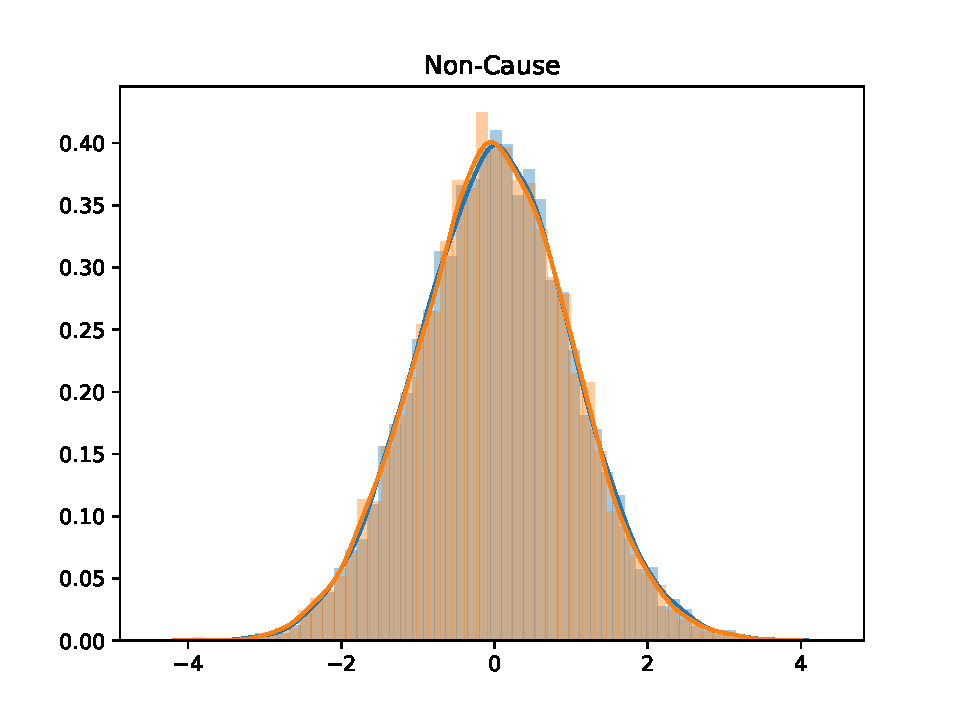
\includegraphics[width=0.5\textwidth]{../src/causality/non-cause}
      \caption{$\Pr^\pol(y_t)$ for $\pol \in \{-1, 1\}$ when $\pol$ is not a cause for $y_t$}
      \label{fig:non-cause-dist}
    \end{figure}
    In this example, it is not the case that $y_t \indep a_t$. Indeed, 
  \end{example}
}
    
    \begin{block}{No confounding}
      \only<article>{We are sure that there is no confounding whenever $y_t \indep \pol \mid a_t$. This is captured by the following diagram.}
      \begin{figure}[H]
        \centering
        \begin{tikzpicture}
          \node[select] at (0,0) (p) {$\pol$};
          \node[RV] at (1,0) (a) {$a_t$};
          \node[RV] at (2,0) (y) {$y_t$};
          \draw[->] (p) to (a);
          \draw[->] (a) to (y);
        \end{tikzpicture}
        \caption{No confounding: $\pol$ causes $y_t$}
        \label{fig:no-confounding}
      \end{figure}
    \end{block}

\only<article>{
  \begin{example}
    Consider the model
    \begin{align*}
      a_t &\sim \Normal(\pol,,1)\\
      y_t \mid a_t, \pol &\sim \Normal(a_t, 1)
    \end{align*}
    \begin{figure}[H]
      \centering
      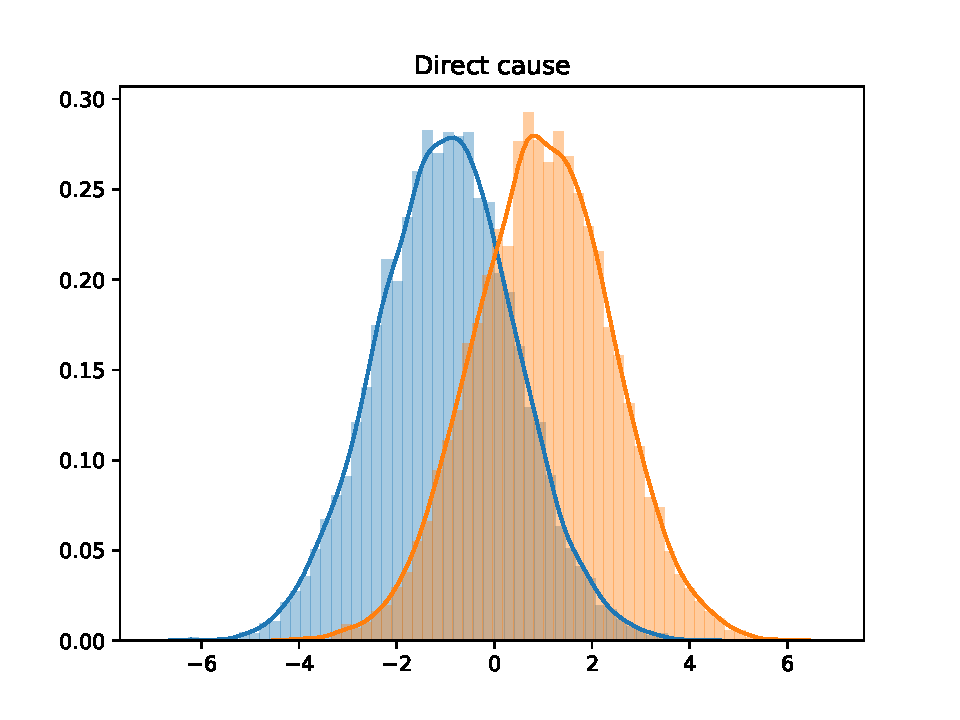
\includegraphics[width=0.5\textwidth]{../src/causality/direct-cause}
      \caption{$\Pr^\pol(y_t)$ for $\pol \in \{-1, 1\}$ when $\pol$ is a direct cause for $y_t$}
      \label{fig:non-cause-dist}
    \end{figure}
  \end{example}
}

  
\end{frame}
\begin{frame}
  \frametitle{Covariates}
  \begin{block}{Sufficient covariate}
  \only<article>{Sometimes the variable of interest is not conditionally independent of the treatment, unless there exists a \emph{sufficient covariate} $x_t$ such that
    $y_t \indep \pol \mid a_t, x_t$. If $x_t$ is not observed, then it is sometimes called a confounder.}
    \begin{figure}[H]
      \centering
      \begin{tikzpicture}
        \node[select] at (0,0) (p) {$\pol$};
        \node[RV] at (1,0) (a) {$a_t$};
        \node[RV] at (2,0) (y) {$y_t$};
        \node[RV] at (2,1) (x) {$x_t$};
        \draw[->] (p) to (a);
        \draw[->] (a) to (y);
        \draw[->] (x) to (a);
        \draw[->] (x) to (y);
      \end{tikzpicture}
      \caption{Sufficient covariate $x_t$}
      \label{fig:sufficient-covariate}
    \end{figure}
  \end{block}

\only<article>{
  \begin{example}
    Consider the model
    \begin{align*}
      x_t &\sim \Normal(0, 1)\\
      a_t &\sim \Normal(x_t + \pol, 1)\\
      y_t \mid a_t, \pol &\sim \Normal(x_t + a_t, 1)
    \end{align*}
    \begin{figure}[H]
      \centering
      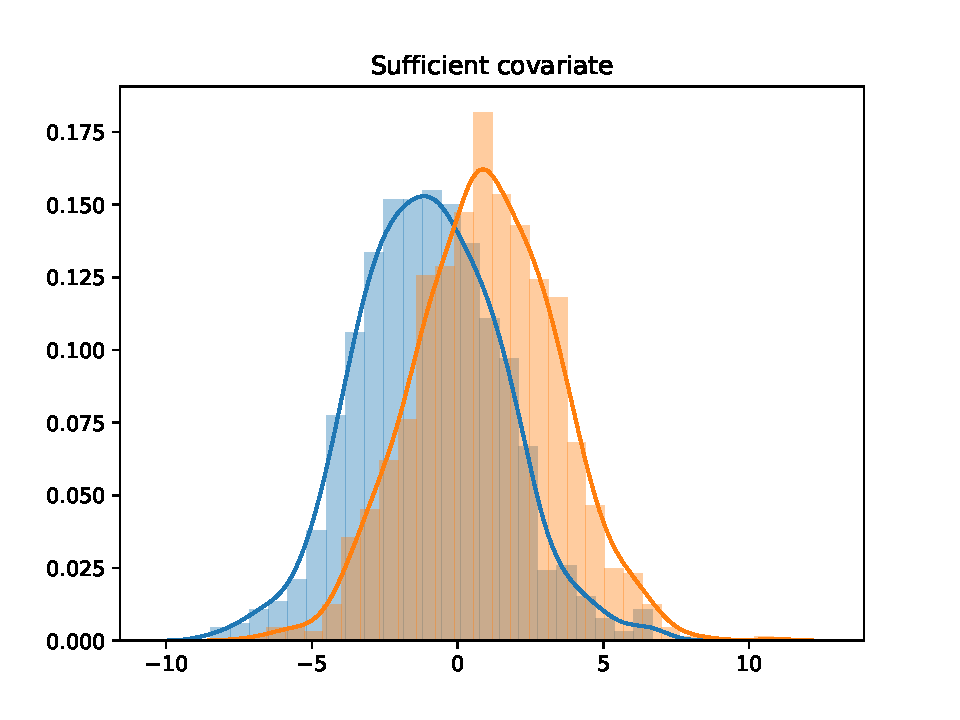
\includegraphics[width=0.5\textwidth]{../src/causality/sufficient}
      \caption{$\Pr^\pol(y_t)$ for $\pol \in \{-1, 1\}$ when $\pol$ is a direct cause for $y_t$}
      \label{fig:non-cause-dist}
    \end{figure}
  \end{example}
}


  \begin{block}{Instrumental variables}
    \only<article>{If the sufficient covariate $x_t$ is not observed, we may still have another variable available, $z_t$, which depends on $x_t$, which is observed, and on the basis of which we make our decisions. However the effect of the treatment depends on $x_t$ directly. This is called an \emph{instrumental variable.}}
    \begin{figure}[H]
      \centering
      \begin{tikzpicture}
        \node[select] at (0,0) (p) {$\pol$};
        \node[RV] at (1,0) (a) {$a_t$};
        \node[RV] at (2,0) (y) {$y_t$};
        \node[RV, hidden] at (2,1) (x) {$x_t$};
        \node[RV] at (1,1) (z) {$z_t$};
        \draw[->] (p) to (a);
        \draw[->] (a) to (y);
        \draw[->] (x) to (y);
        \draw[->] (x) to (z);
        \draw[->] (z) to (a);
      \end{tikzpicture}
      \caption{Instrumental variable $z_t$}
      \label{fig:instrumental-variable}
    \end{figure}
  \end{block}

\only<article>{
  \begin{example}
    Consider the model
    \begin{align*}
      x_t &\sim \Normal(0, 1)\\
      z_t &\sim \Normal(x_t, 1)\\
      a_t &\sim \Normal(z_t + \pol, 1)\\
      y_t \mid a_t, \pol &\sim \Normal(x_t + a_t, 1)
    \end{align*}
    \begin{figure}[H]
      \centering
      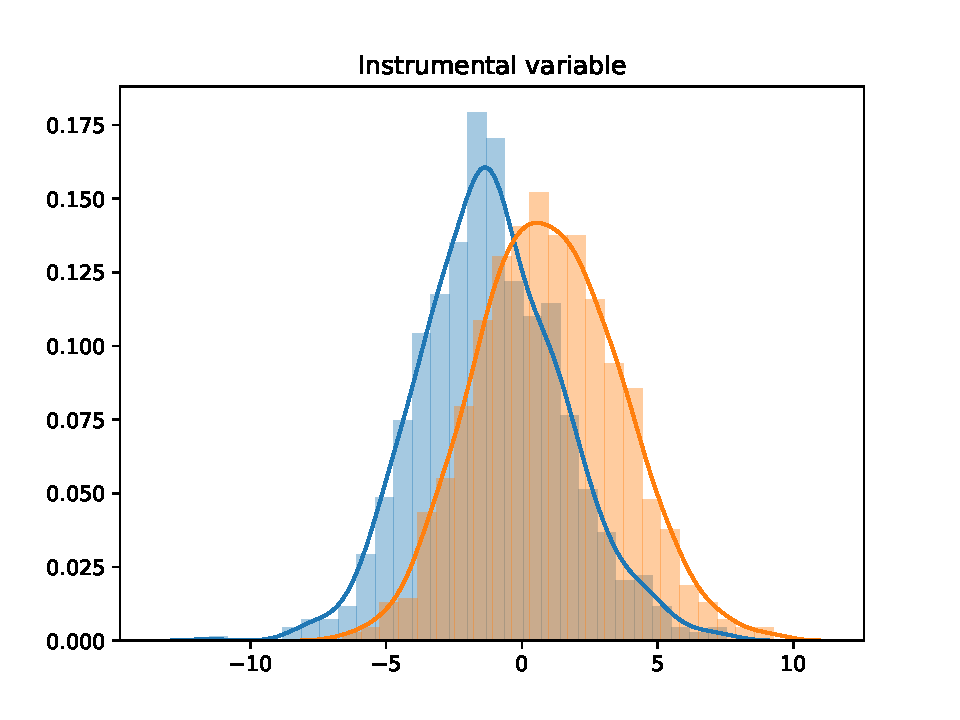
\includegraphics[width=0.5\textwidth]{../src/causality/instrumental}
      \caption{$\Pr^\pol(y_t)$ for $\pol \in \{-1, 1\}$ when $\pol$ is a direct cause for $y_t$}
      \label{fig:non-cause-dist}
    \end{figure}
  \end{example}
}


\end{frame}


\subsection{Interventions}
\only<article>{Interventions are of primary interest when we have a set of observational data, collected under a \emph{null} or \emph{default} policy $\pol_0$.  We then wish to intervene with some policy $\pol$ in order to maximise our utility function, or to simply try and estimate the exact relationships between variables.}
\begin{frame}
  \begin{example}[Weight loss]
    \only<article>{Consider weight loss. We can collect observational data from a population of overweight adults over a year. We can imagine that $x$ represents the weight and vital statistics of an individual and $y$ their change in weight after a year. We may also observe their individual actions $a$, such as whether or not they are following a particular diet or exercise regime. Under the default policy $\pol_0$, their actions are determined only the individuals. Consider an alternative policy $\pol$, which prescribes diet and exercise regimes. Due to non-compliance, actual actions taken by individuals may differ from prescribed actions.}
    \begin{figure}[H]
      \centering
      \begin{tikzpicture}
        \node[RV] at (0,0) (x) {$x$};
        \node[RV] at (1,1) (y) {$y$};
        \node[RV] at (2,0) (a) {$a$};
        \draw[->] (x)--(y);
        \draw[->] (x)--(a);
        \draw[->] (a)--(y);
        \node[select] at (4,0) (p) {$\pol$};
        \draw[->] (p)--(a);
        \node[utility] at (3,1) (u) {$\util$};
        \draw[->] (a)--(u);
        \draw[->] (y)--(u);
      \end{tikzpicture}
    \end{figure}
  \end{example}
\end{frame}  


\subsection{Instrumental variables}
\begin{frame}
  \begin{example}
    \begin{figure}[H]
      \centering
      \begin{tikzpicture}
        \node[RV] at (0,0) (x) {$x$};
        \node[RV] at (1,0) (y) {$y$};
        \node[RV] at (0,1) (z) {$z$};
        \node[RV] at (1,1) (p) {$p$};
        \node[RV,hidden] at (2,0) (o) {$\omega$};
        \draw[->] (x) to (y);
        \draw[->] (x) to (p);
        \draw[->] (z) to (p);
        \draw[->] (p) to (y);
        \draw[->] (o) to (p);
        \draw[->] (o) to (y);
      \end{tikzpicture}
    \end{figure}
  \end{example}
\end{frame}
\subsection{Confounders}
\begin{frame}
  \begin{example}[Weight loss]
    \begin{figure}[H]
      \centering
      \begin{tikzpicture}
        \node[RV] at (0,0) (x) {$x$};
        \node[RV] at (1,1) (y) {$y$};
        \node[RV] at (2,0) (a) {$a$};
        \draw[->] (x)--(y);
        \draw[->] (x)--(a);
        \draw[->] (a)--(y);
        \node[select] at (4,0) (p) {$\pol$};
        \draw[->] (p)--(a);
        \node[utility] at (3,1) (u) {$\util$};
        \draw[->] (a)--(u);
        \draw[->] (y)--(u);
        \node[RV, hidden] at (0,2) (c) {$c$};
        \draw[->] (c)--(y);
      \end{tikzpicture}
    \end{figure}
  \end{example}
\end{frame}  

\subsection{Inference in causal models}

\only<article>{Inference in causal models requires building a complete model for the effect of every action.}

\section{Counterfactual analysis}

\only<article>{
Counterfactual analysis is mainly about questions relative to individuals, and specifically about what the effects of alternative actions would have been in the past. 
}
\subsection{Disturbances and structural equation models}

\begin{frame}
  \only<article>{A structural equation model describes the random variables as deterministic functions of the decisions variables and the random exogenous disturbances. This allows us to separate the unobserved randomness from the known functional relationship between the other variables. Structurally, the model is essentially a variant of decision diagrams, as shown in Figure~\ref{fig:disturbance-model}.}
  \begin{figure}[H]
    \centering
    \begin{tikzpicture}
      \node[RV, hidden] at (-1,1) (p) {$\param$};
      \node[RV] at (0,0) (x) {$x_t$};
      \node[RV] at (1,1) (y) {$y_t$};
      \node[RV] at (2,0) (a) {$a_t$};
      \draw[->] (x)--(y);
      \draw[->] (x)--(a);
      \draw[->] (a)--(y);
      \draw[->] (p) to (x);
      \draw[->] (p)--(y);
      \node[select] at (4,0) (pol) {$\pol$};
      \draw[->] (pol)--(a);
      \node[utility] at (3,1) (u) {$\util$};
      \draw[->] (a)--(u);
      \draw[->] (y)--(u);
      \node[RV, hidden, above of=y]  (oy) {$\omega_{t,y}$};
      \node[RV, hidden, below of=x]  (ox) {$\omega_{t,x}$};
      \node[RV, hidden, below of=a]  (oa) {$\omega_{t,a}$};
      \draw[->] (ox) -- (x);
      \draw[->] (oa) -- (a);
      \draw[->] (oy) -- (y);
    \end{tikzpicture}
    \caption{Decision diagram with exogenous disturbances $\omega$.}
    \label{fig:disturbance-model}
  \end{figure}
  \only<article>{We still need to specify particular functional relationships between the variables. Generally speaking, a random variable taking values in $\CX$, is simply a function $\Omega \times \Param \to \CX$. For example, in Figure~\ref{fig:disturbance-model} $y_t = f_y(\omega, \theta)$. Taking into account the dependencies, this can be rewritten in terms of a function of the other random variables, and the local disturbance: $y_t = f_{y|a,x}(a,x, \omega_{t,y}, \theta)$. The choice of the function, together with the distribution of the parameter $\param$ and the disturbances $\omega$, fully determines our model.}
  \begin{example}[Structural equation model  for Figure~\ref{fig:disturbance-model}]
    \only<presentation>{\vspace{-1em}}
    \only<article>{
      In structural equation models, the only random variables are the exogenous disturbances. In a fully Bayesian framework, $\param$ is also a latent random variable. The remaining variables are  deterministic functions. 
    }
    \begin{align*}
      \theta &\sim \Normal(\vectorsym{0}_4, \eye_4),\\
      x_t &= \theta_0 \omega_{t,x},
          & \omega_{t,x} &\sim \Bernoulli(0.5)\\
      y_t &= \theta_1 y_t + \theta_2 x_t + \theta_3 a_t + \omega_{t,y},
          &\omega_{t,y} &\sim \Normal(0,1)\\
      a_t &= \pol(x_t) + \omega_{t,a} \mod |\CA| 
          &\omega_{t,a} &\sim 0.1 \Singular(0) + 0.9 \Uniform(\CA),
    \end{align*}
  \end{example}
  \only<article>{Structural equation models are particularly interesting in applications such as economics, where there are postulated relations between various economic quantities. }
\end{frame}

\begin{frame}
  \frametitle{Treatment-unit additivity}
  
\end{frame}



\section{Application to recommendation systems}
\begin{frame}

  \only<2>{
    \only<article>{If we have data $D = \cset{(x_t, a_t, y_t)}{t \in [T]}$ generated from some policy $\pol_0$, we can always infer the average quality of each action $a$ under that policy.}
    \begin{align}
      \label{eq:observed-expected-utility}
      \hat{\E}_D(U \mid a) 
      &\defn
        \frac{1}{|\cset{t}{a_t = a}|}
        \sum_{t: a_t = a}
        U(a_t, y_t)
        \approx
        \E^{\pol_0}_\param (U \mid a).
    \end{align}
  }
  \only<article>{
    Can we calculate the value of another policy? As we have seen from Simpson's paradox\index{Simpson's paradox}, it is folly to simply select
    \[
    \hat{a}^*_D \in \argmax_a \hat{\E}_D(U \mid a),
    \]
    as the action also depends on the observations $x$ through the policy.
    To clarify this, let us define the model shown in Figure~\ref{fig:recommendation-decision-diagram}.
    \begin{align*}
      x_t \mid \param, x_t &\sim P_\param(x)\\
      y_t \mid \param, x_t, a_t &\sim P_\param(y \mid x_t, a_t)\\
      a_t \mid x_t, \pol &\sim \pol(a \mid x_t).
    \end{align*}
    Assume that $x \in \CX$, a continuous space, but $y \in \CY$ is discrete. Then the value of an action under a policy $\pol$ is
    \begin{align*}
      \E^\pol_\param(\util \mid a)
      &=
        \int_\CX \dd P_\param(x)
        \sum_{y \in \CY} P_\param(y \mid x, a) \util(a, y).
    \end{align*}
    We see that there is a clear dependence on the distribution of $x$, and there is no dependence on the policy any more. In fact, equation above only tells us the expected utility we'd get if we always chose the same action $a$. But what is the optimal policy? First, we have to define the value of a policy.
  }
  
  \begin{block}{The value of a policy}
    \begin{align*}
      \E^\pol_\param(\util)
      &=
        \int_\CX \dd P_\param(x)
        \sum_{y \in \CY} P_\param(y \mid x, a) \util(a, y) \sum_{a \in \CA} \pol(a \mid x).
    \end{align*}
  \end{block}
  \only<article>{
    The optimal policy under a known parameter $\param$ is given simply by
    \begin{align*}
      \max_{\pol \in \Pol} \E^\pol_\param(\util),
    \end{align*}
    where $\Pol$ is the set of allowed policies. How can we actually find the optimal policy?
  }
\end{frame}


\subsection{Discussion}
\begin{frame}
  \begin{block}{Further reading}
    \begin{itemize}
    \item Pearl, \emph{Causality}.
    \item \citet{dawid2012decision}
    \end{itemize}
  \end{block}
\end{frame}
%%% Local Variables:
%%% mode: latex
%%% TeX-engine: xetex
%%% TeX-master: "notes"
%%% End:
